%-- Add sections and your outline will be created automatically --%
\section{Flow past a sphere}

% Frame starts a new slide
\begin{frame}
    \frametitle{Flow past a sphere}
\begin{itemize}
\item Drag calculation at different Reynolds numbers
\item Adaptive mesh resolves dynamics near surface
%\item Option: \option{Velocity/stat/compute\_body\_forces\_on\_surfaces}
\end{itemize}
\begin{figure}
\centering
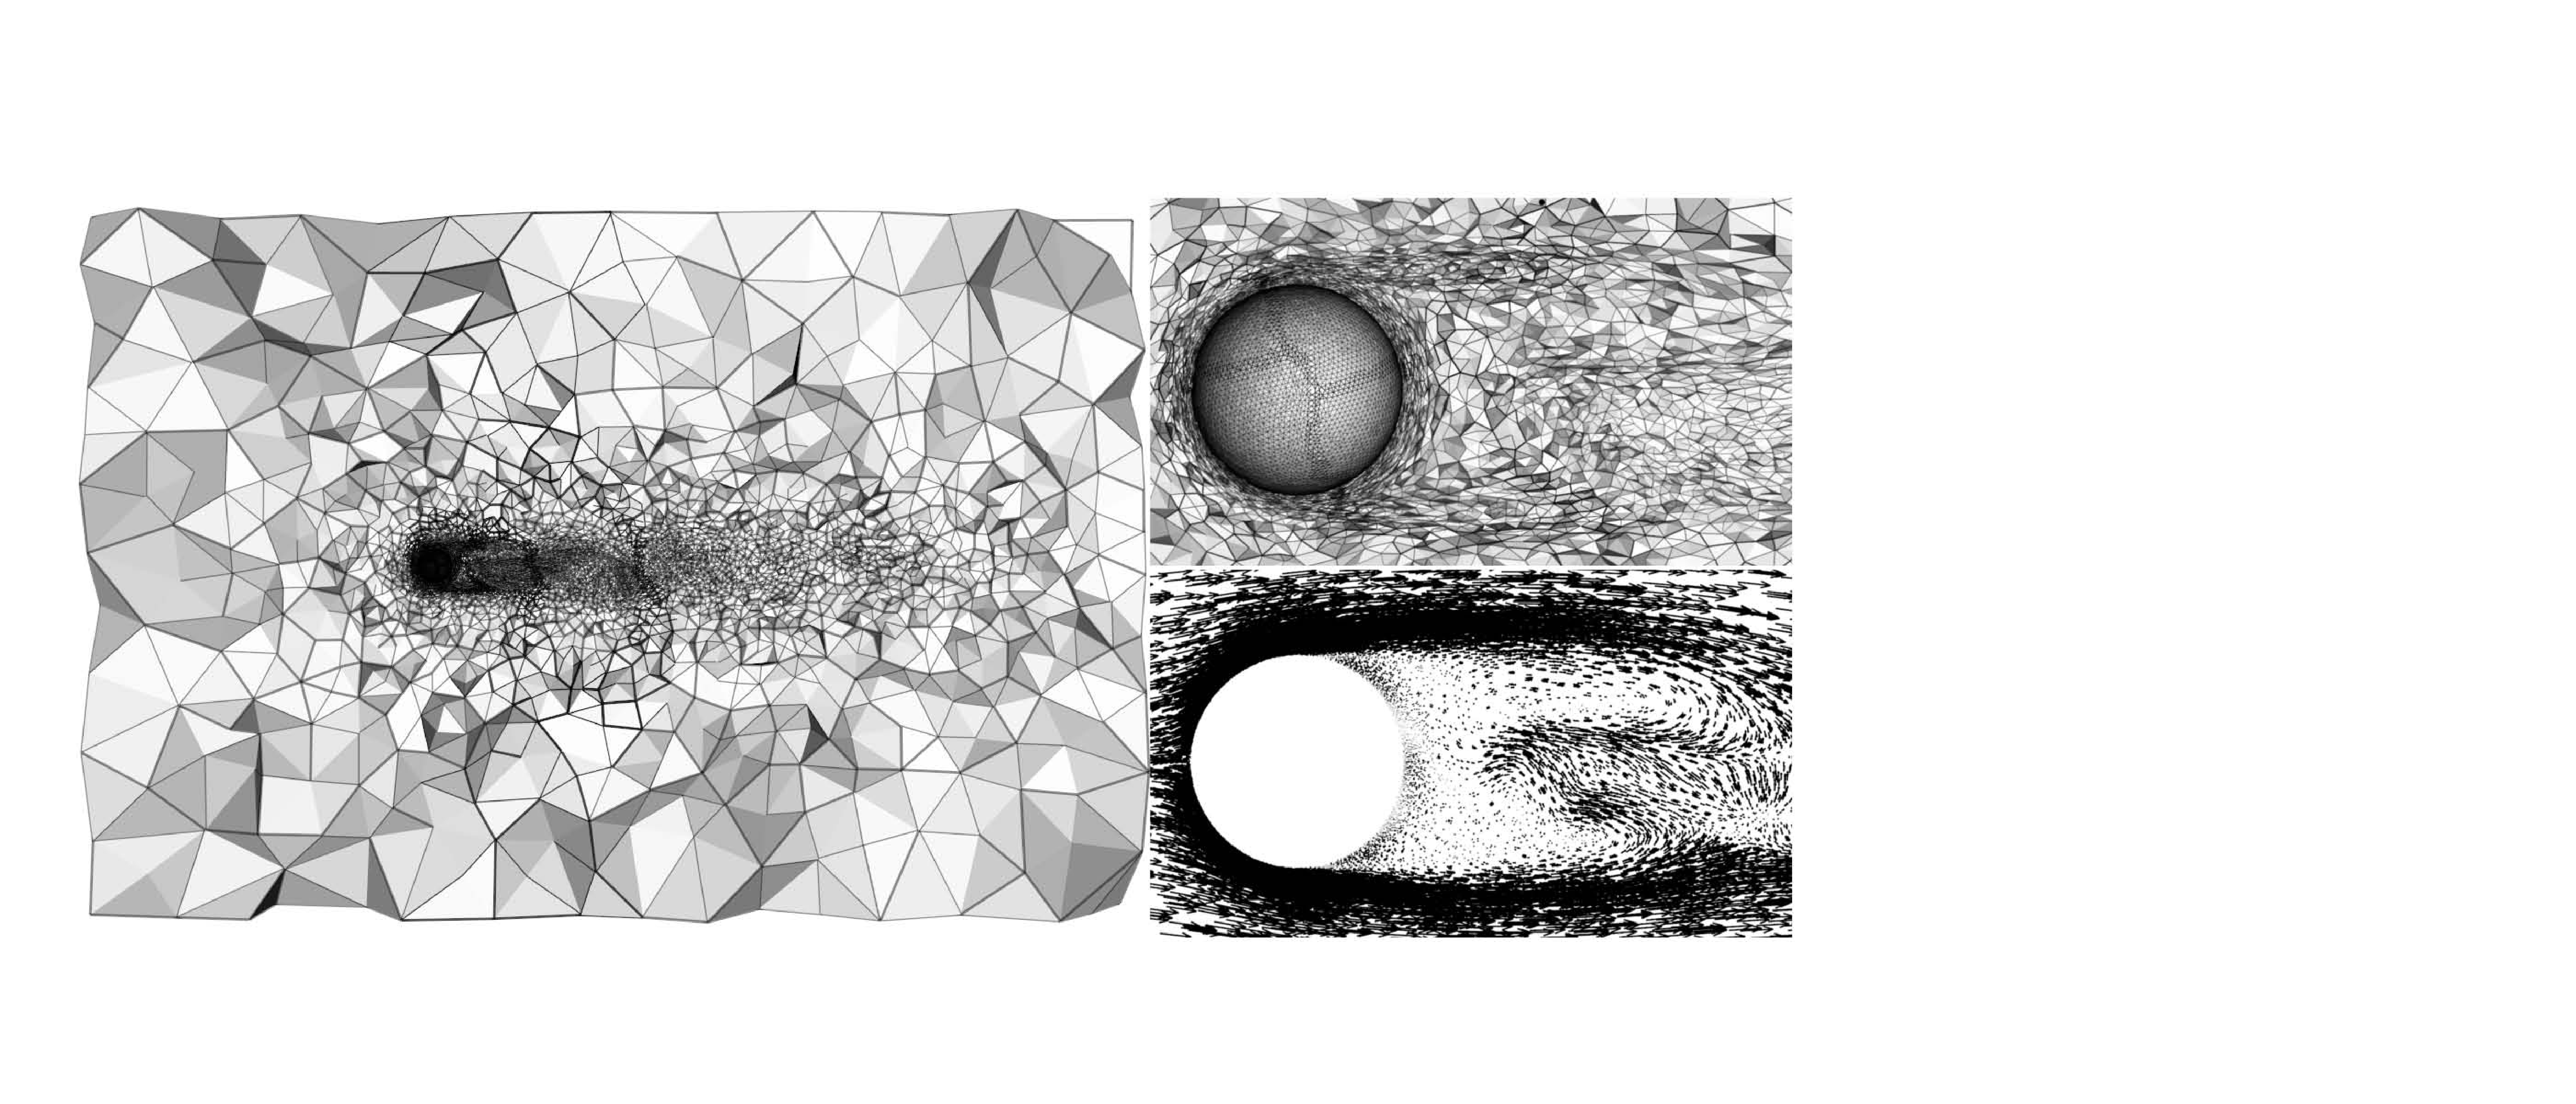
\includegraphics[width=0.8\textwidth]{./flow_past_sphere/sphere-Re1000-combined.pdf}
\caption{Sphere at $Re = 1000$. Clockwise from left: Cut plane showing anisotropic mesh, close up of sphere, velocity vectors.}
\end{figure}
\end{frame}

\begin{frame}
    \frametitle{Flow past a sphere}
\begin{itemize}
\item Plot streamlines by processing vtu files in Paraview
\item Time series of pressure and viscous drag force integrals available in stat file
%\item Option: \option{Velocity/stat/compute\_body\_forces\_on\_surfaces}
\end{itemize}
\begin{figure}
\centering
\subfigure[Re = 1]{
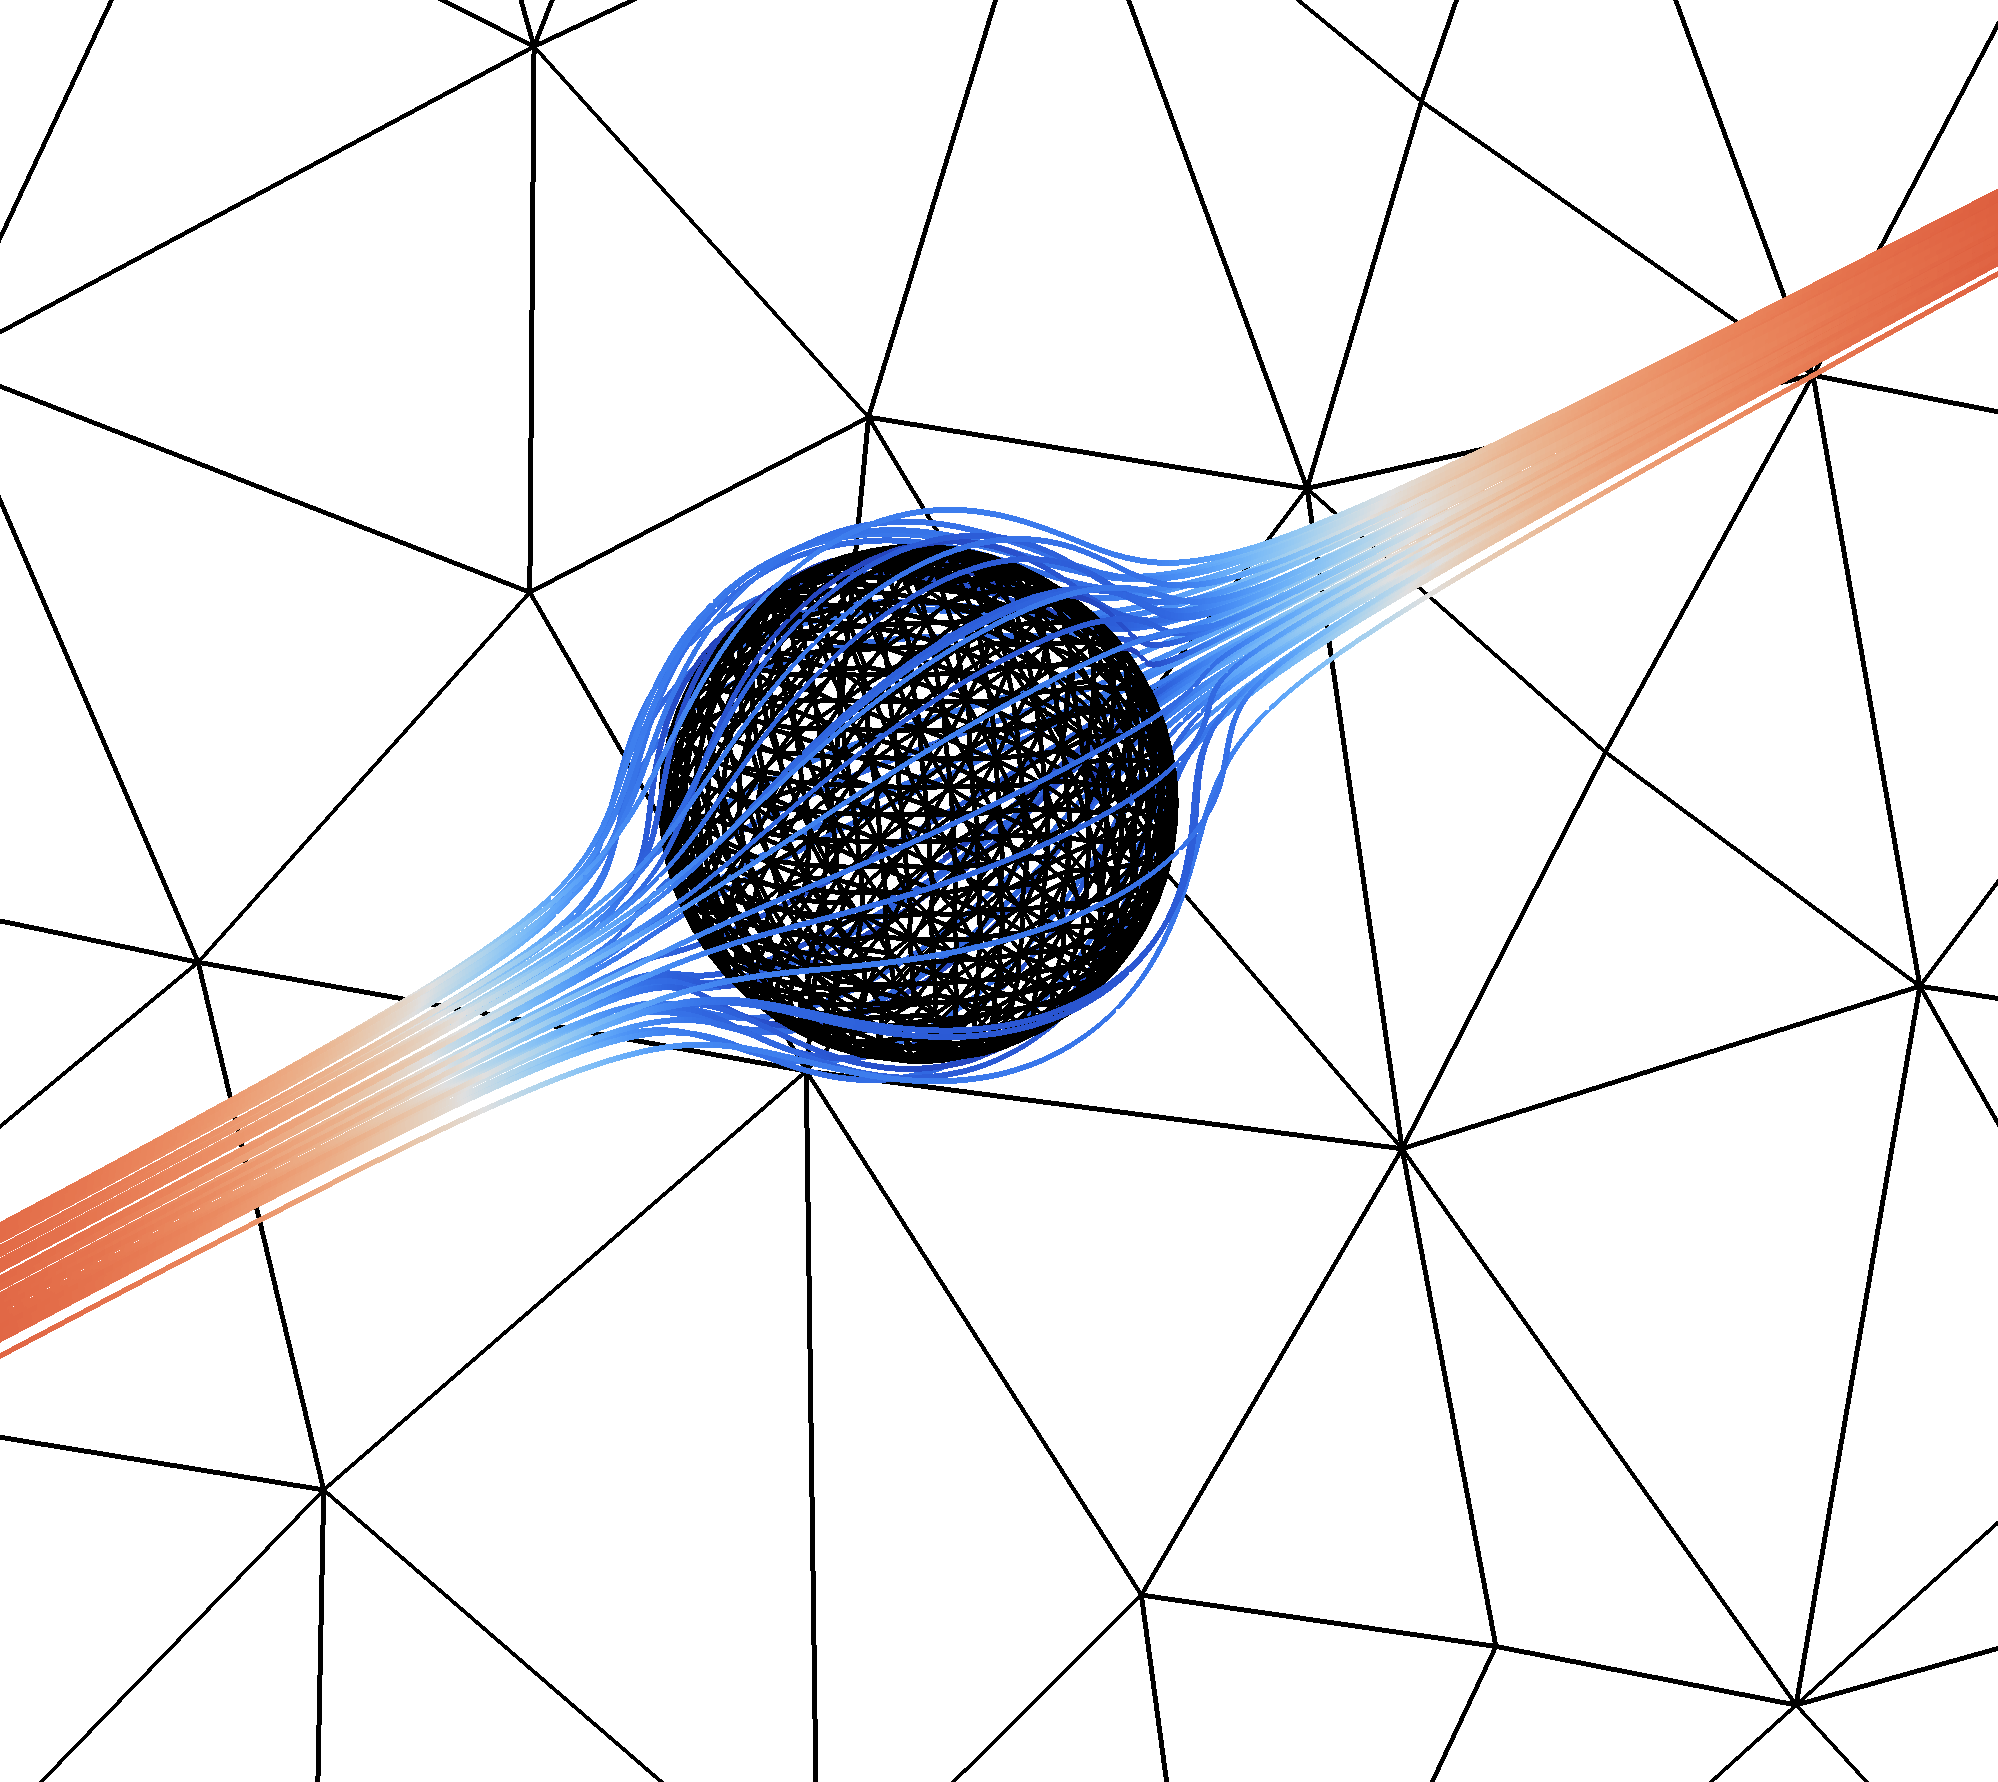
\includegraphics[width=0.225\textwidth]{./flow_past_sphere/sphere-Re1-streamlines.png}}
\subfigure[Re = 10]{
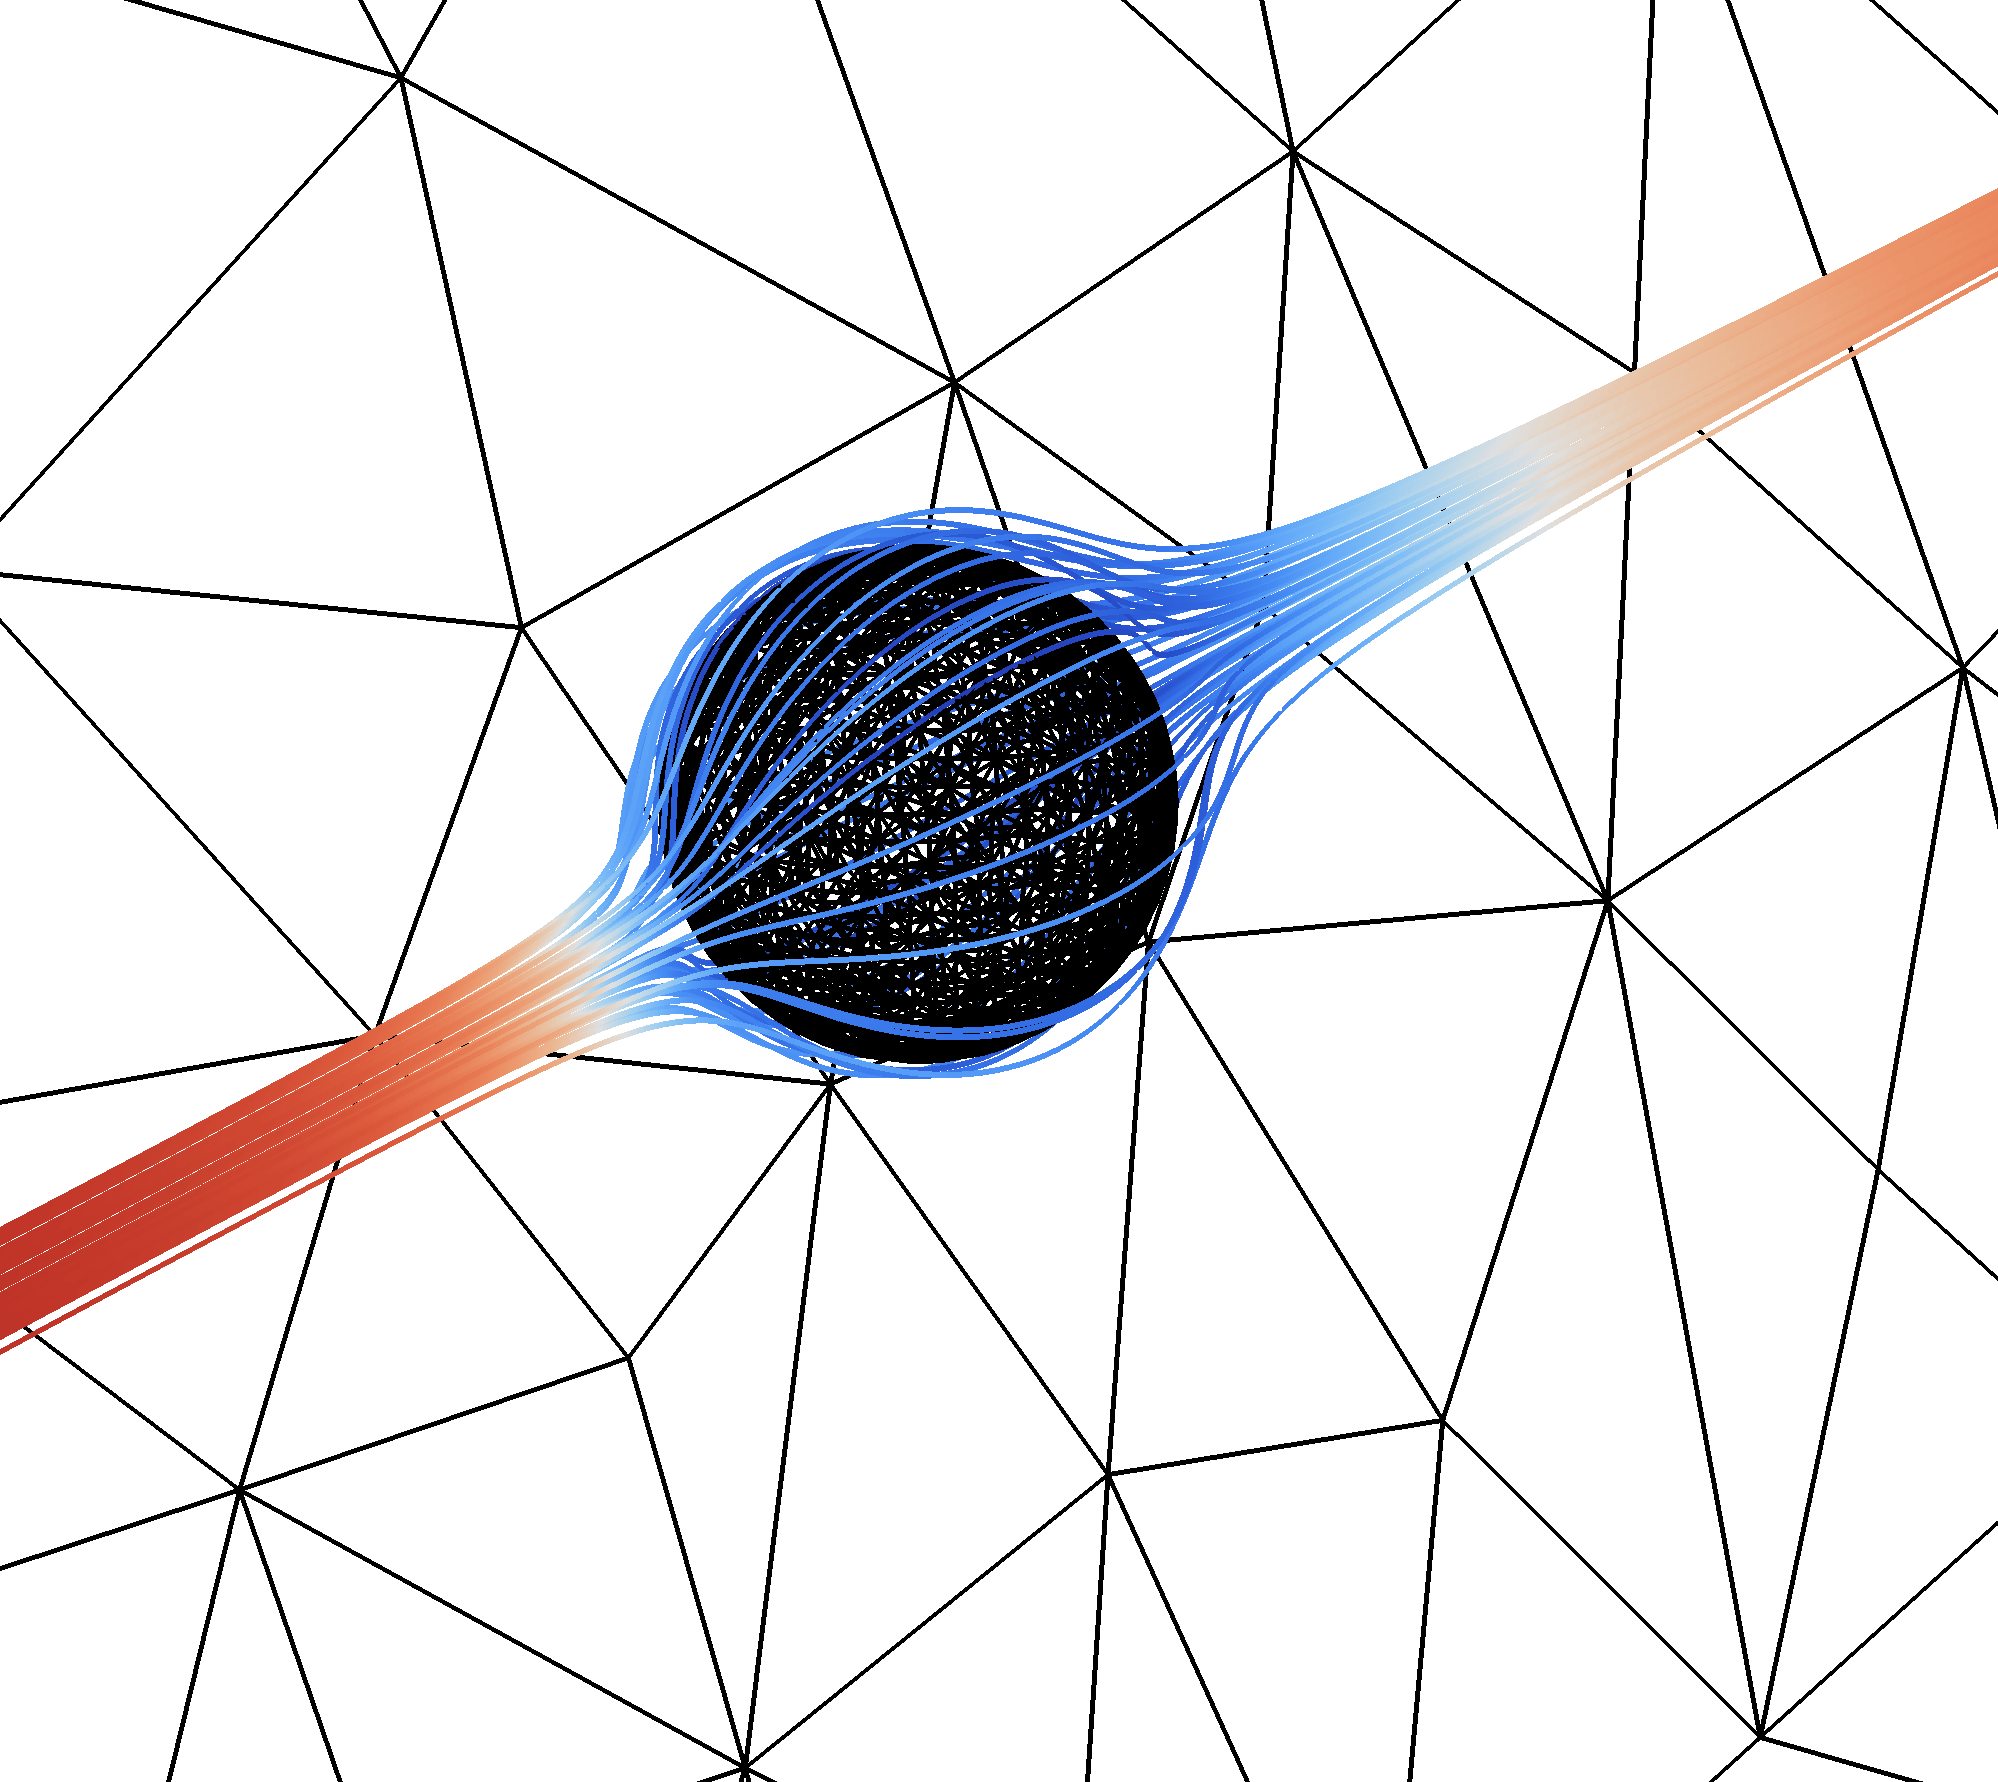
\includegraphics[width=0.225\textwidth]{./flow_past_sphere/sphere-Re10-streamlines.png}}
\subfigure[Re = 100]{
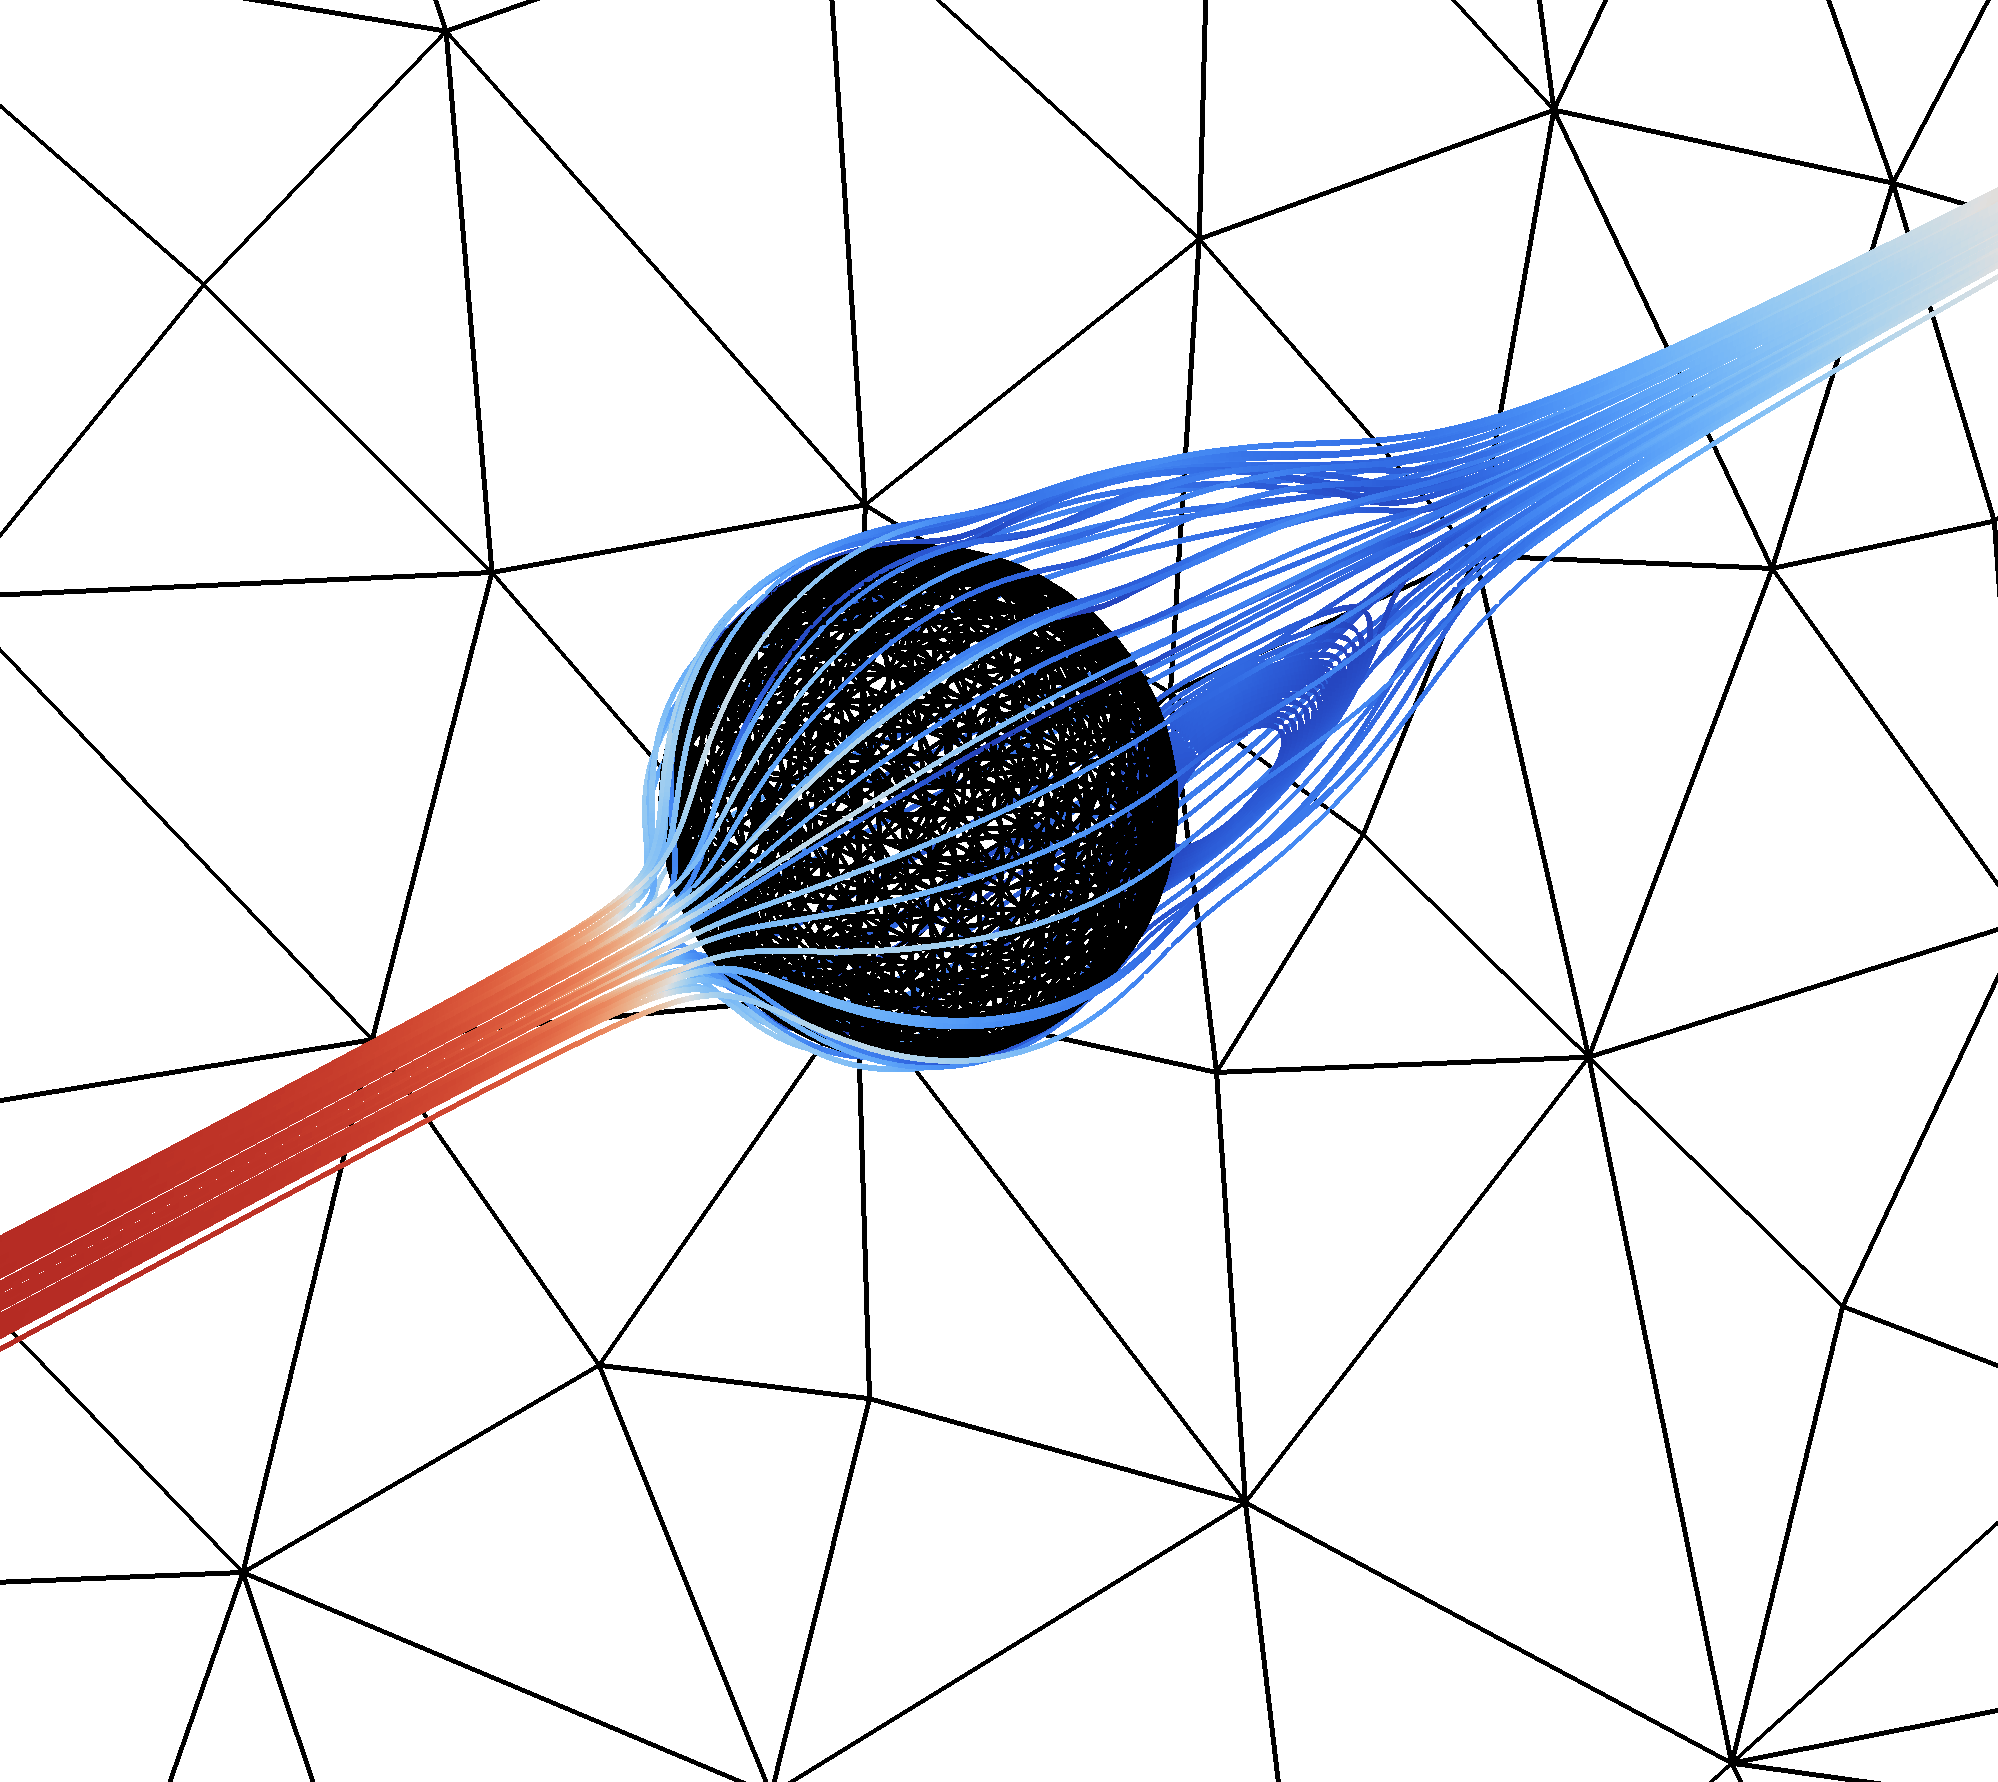
\includegraphics[width=0.225\textwidth]{./flow_past_sphere/sphere-Re100-streamlines.png}}
\subfigure[Re = 1000]{
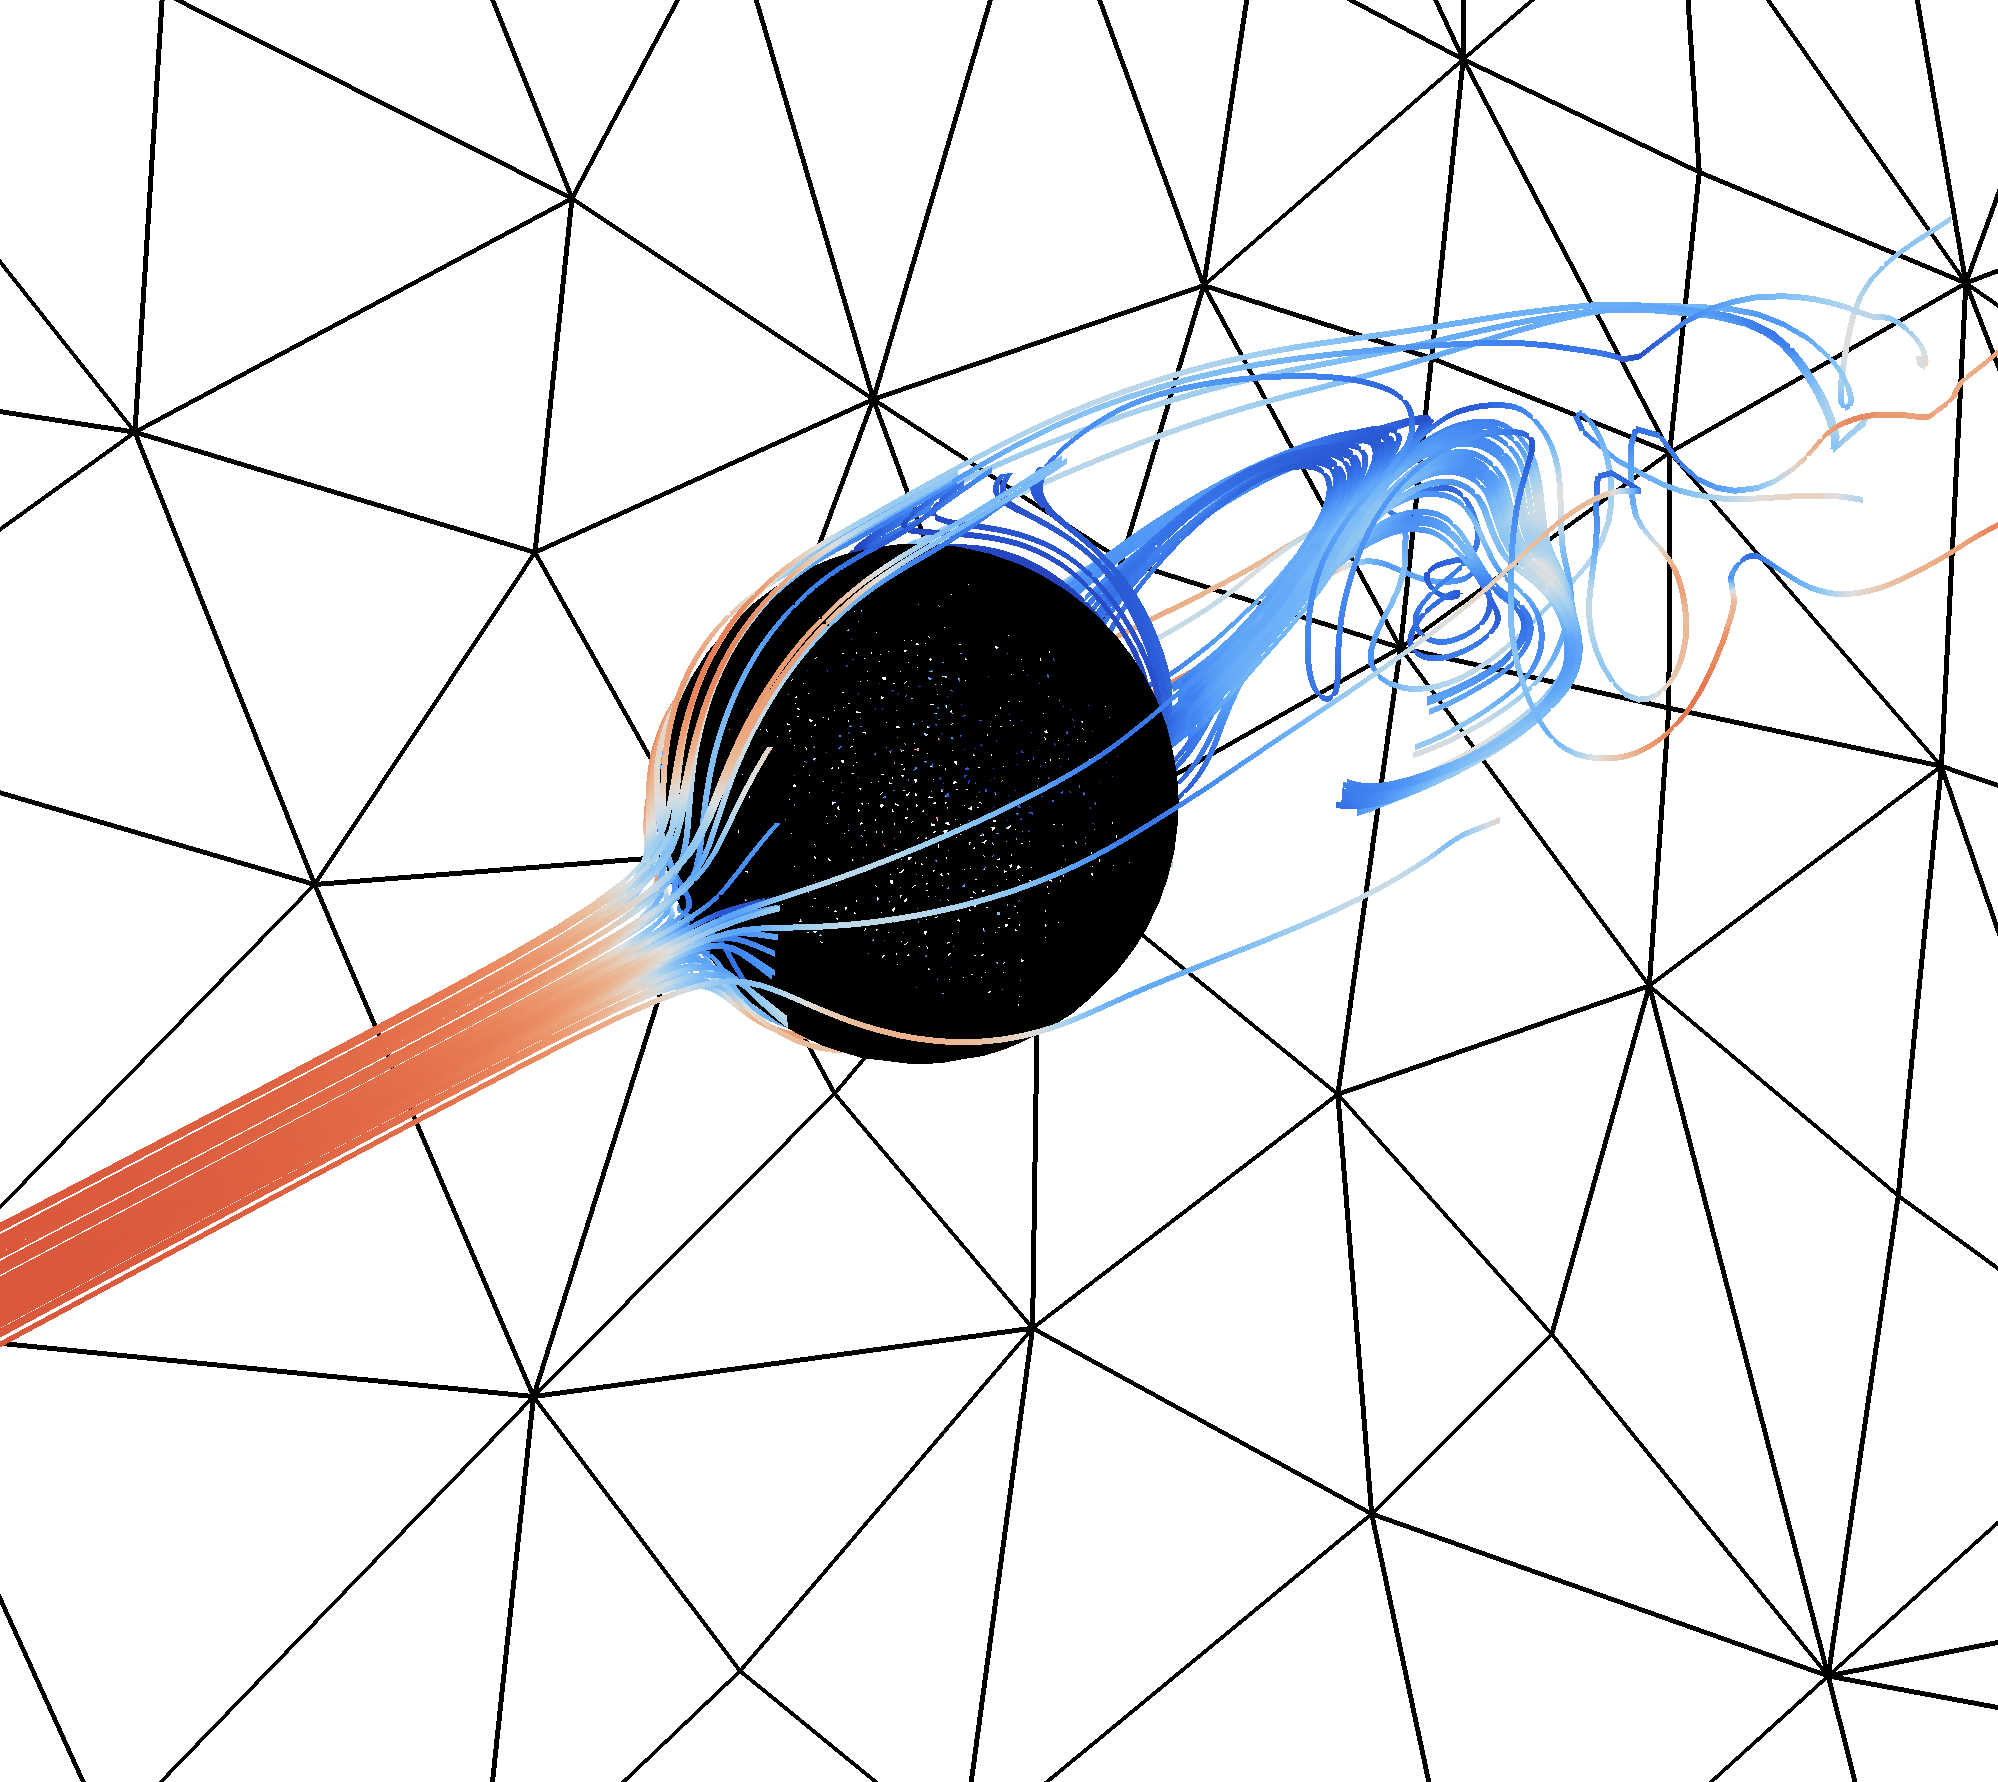
\includegraphics[width=0.225\textwidth]{./flow_past_sphere/sphere-Re1000-streamlines.png}}
\caption{Streamlines showing transition from laminar to turbulent wake with increasing Reynolds number.}
\end{figure}
\end{frame}

\begin{frame}
    \frametitle{Flow past a sphere}
\begin{figure}
\centering
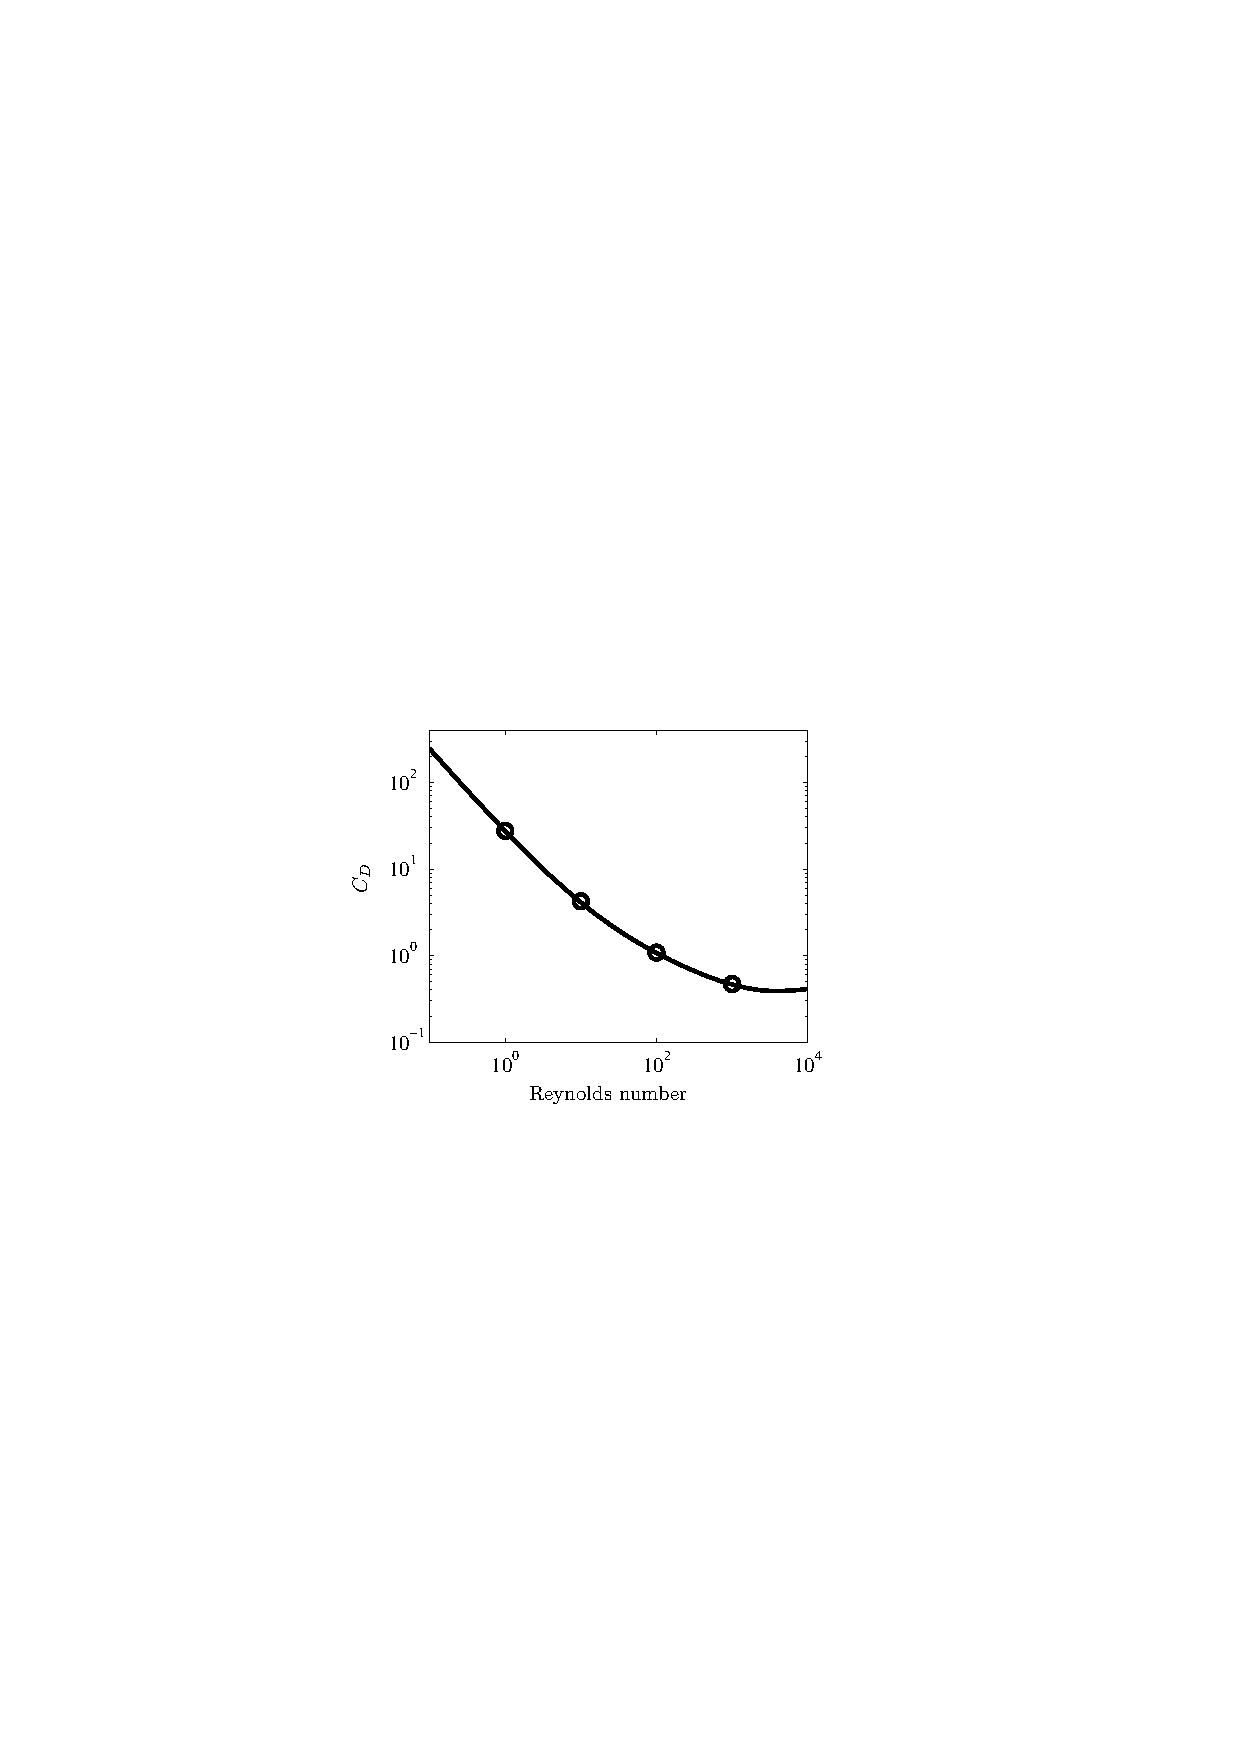
\includegraphics[width=0.5\textwidth]{./flow_past_sphere/Sphere_Drag.pdf}
\caption{Plot of drag coefficient vs. Reynolds number showing effect of turbulence. Circles: Fluidity data, line: correlation to experimental data from Brown and Lawler (2003), Journal of Environmental Engineering, 129(3).}
\end{figure}
\end{frame}

\begin{frame}
\frametitle{Flow past a sphere, exercises}
\begin{itemize}
\item Write an offline python diagnostic to calculate the drag.
\item Investigate impact different discretisations and adaptivity parameters on the drag.
\item Investigate different shaped objects.
\end{itemize}
\end{frame}
